\chapter{Implémentations et synthèse de texture}
\label{chap:chapitre2}

Notre recherche est une étude exploratoire du modèle multi-résolutionnel local, en particulier de la congruence de phase, issu du traitement d'images, appliquée dans le contexte de la synthèse de texture. Nous allons maintenant voir la mise en application des concepts exposés à la partie précédente, ainsi que les résultats obtenus.

\section{Implémentation}

Les concepts d'énergie locale et de signal monogène ne sont pas des notions communément utilisées dans le traitement d'images, aucune librairie standard ne les implémente à notre connaissance. Nous avons donc dû implémenter nous-même les algorithmes pour mettre en place le modèle multi-résolutionnel local. Le choix du logiciel pour faire ces implémentations a été une question importante.


%\subsection{OpenCV}
\paragraph{OpenCV}

Malgré notre but final de travailler sur de la synthèse de texture, nous avons commencé par développer un petit logiciel pour pouvoir itérer rapidement et expérimenter avec les concepts de base du modèle multi-résolutionnel local sur des images, sans prendre en compte les problématiques de la synthèse. Pour cela, nous mis au point un logiciel utilisant \cpp avec la librairie OpenCV~\cite{opencv_library}. OpenCV est une librairie standard de traitement d'images en temps réel et de vision par ordinateur, disponible pour les langages de programmation \cpp, Python et Java. Les images y sont représentées comme des matrices, et les opérations de bas niveau courantes du traitement d'images y sont implémentées, comme la lecture, l'écriture, l'affichage, le filtrage, la convolution, et autres.  Notre logiciel permet à un utilisateur de créer, visualiser, et modifier les pyramides d'une image d'entrée, ainsi que de calculer et visualiser la congruence de phase. Avec ces fonctionnalités, nous avons fait des expérimentations pour voir l'effet de différentes modifications et reconstructions de la pyramide de Riesz d'une image.


\bigskip

Plusieurs raisons ont ensuite motivé notre choix de changer d'implémentation. Après avoir expérimenté avec la congruence de phases sur des images, nous voulions travailler avec des textures, c'est à dire faire de la synthèse dans le cadre du pipeline graphique traditionnel. Plus que simplement reconstruire une image, nous voulions maintenant synthétiser une texture à projeter sur une surface, potentiellement infinie, dans le but de la recouvrir. Dans un tel contexte, plusieurs problématiques surviennent. La synthèse de texture doit pouvoir se faire dans le fragment shader, depuis le GPU, pour être mise en place dans le pipeline graphique. Cela veut dire avoir une méthode de reconstruction parallélisable, ce qui n'est pas le cas de la méthode que nous utilisions jusque là. Se posent aussi des questions de projection et de filtrage, que n'avions pas eu à traiter jusque là, mais nécessaires à considérer pour de la synthèse de textures.

Parallèlement, notre laboratoire de recherche a accueilli de nouveaux membres, qui travaillaient sur des problématiques similaires aux nôtres. Nous voulions alors mettre en place un logiciel qui servirait de base de travail commune pour les personnes faisant de la synthèse de textures dans le laboratoire. Nous avons considéré plusieurs options, notamment développer un moteur de rendu personnalisé et adapté à nos besoins, ou utiliser un des moteurs de jeu Unity3D~\cite{unity_engine} ou Unreal Engine~\cite{unreal_engine}. Le problème d'un moteur personnalisé est qu'il nous aurait fallu réimplémenter beaucoup de choses nous-même, ce qui aurait été long et redondant. Les moteurs Unity3D et Unreal Engine, eux, avaient le désavantage de ne pas offrir la flexibilité de manipuler les textures tel que nous souhaitions le faire. Nous avons donc choisi une autre option, le moteur de jeu Godot~\cite{godot_game_engine}.

\paragraph{Godot}

Godot est un logiciel libre et gratuit, moteur de jeu 2D et 3D, qui permet de faire du rendu temps-réel et donc de s'intéresser aux problématiques de la synthèse de texture, ce que ne permettait pas OpenCV. Bien que pour l'instant moins populaire que Unity et Unreal Engine, Godot est une solution qui croit en notoriété, surtout dans la recherche en informatique graphique, car il est léger et flexible, et permet facilement d'écrire des modules personnalisés ou de modifier du code source pour s'adapter aux besoins des utilisateurs. C'est ce que nous avons fait avec Nicolas Lutz, post-doctorant du laboratoire. Nous avons travaillé conjointement à développer \textit{TexSyn}, une librairie \cpp de traitement d'images et de synthèse de texture pour Godot.

Godot a une classe qui gère les textures, mais la manipuler est compliqué et peu efficace pour des opérations d'accès direct dont nous avons besoin pour nos synthèses. Notre librairie \textit{TexSyn} définit donc une classe d'image plus pratique à utiliser, avec toutes les opérations dont nous avons besoin, qui est ensuite interfacée avec la classe d'image de Godot pour être utilisée depuis l'éditeur. On construit SY avec cela nos pyramides en pré-calcul sur le CPU, que l'on stocke dans des atlas de textures, qui sont ensuite chargés sur le GPU. On fait alors la reconstruction depuis nos shaders, en temps réel, en utilisant les pyramides stockées dans les atlas. Cette reconstruction a cependant des problèmes de filtrage, car nous ne pouvons pas appliquer de convolution avec un filtre pour faire un lissage depuis le fragment shader. Nous avons ensuite travaillé à développer une méthode de synthèse pouvant traiter des textures à structure irrégulière, en mettant au point un échantillonneur préservant la congruence de phases, détaillé plus loin dans ce chapitre.

\begin{figure}
    \centering
    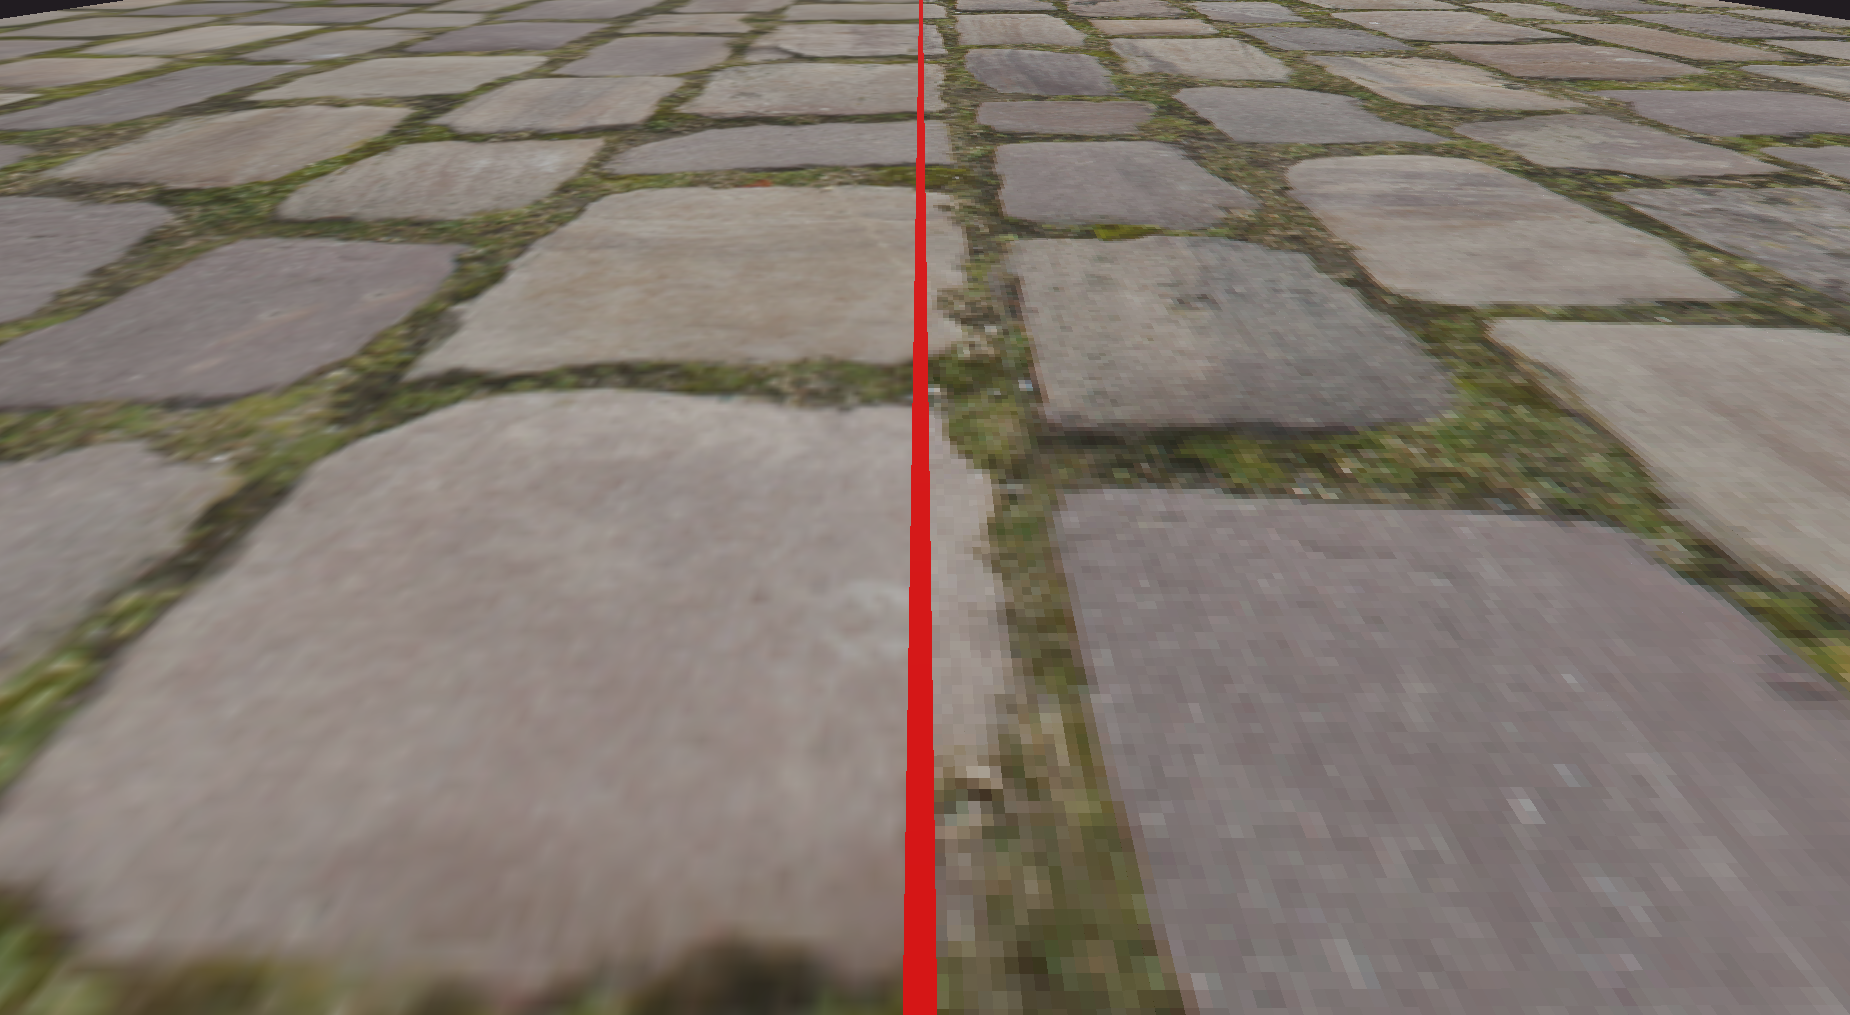
\includegraphics[width=0.9\textwidth]{contenu/resources/images/reconstruction_cpu_vs_gpu}
    \caption[Reconstruction de texture dans \textit{TexSyn}]{Reconstruction de la pyramide de Riesz d'une texture, hors-ligne depuis le CPU (gauche) et en temps-réel depuis le fragment shader (droite). On remarque les artefacts de filtrage sur la reconstruction en temps-réel)}
    \label{fig:texsyn-reconstruction}
\end{figure}


\section{Sélection de niveaux de fréquences}

La mise au point de la congruence de phases et l'utilisation d'un contexte multi-résolutionnel nous ont permis de visualiser explicitement que les différents niveaux de structure que l'on trouve dans une image sont liés à différents niveaux de d'échelle. Nous avons émis l'hypothèse que chaque niveau de structure que l'on distingue dans une image peut s'exprimer comme la congruence en phases d'un sous-ensemble fréquentiel. Autrement dit, chaque échelle de structure est créée par un sous-ensemble de niveaux de la pyramide d'image. Pour vérifier cela, nous avons regardé quel était le résultat de sélectionner seulement certains sous-ensembles de niveaux de la pyramide et de calculer la congruence de phases sur ces niveaux.

\begin{equation}
    PC_{\mathcal{S}}(\mathbf{x}) = \frac{W(x)E(\mathbf{x})}{\epsilon + \sum_{n\in\mathcal{S}} A_{n}(\mathbf{x})},
\end{equation}

où $\mathcal{S}$ est un sous-ensemble de niveaux de la pyramide. En pratique, nous avons essayé avec tous les $\mathcal{S} = \llbracket a, b\rrbracket$ avec $1 \leq a \leq b \leq d$. Cela nous a permit de confirmer que les différents niveaux de structure étaient bien causés par différents sous-ensembles fréquentiels, comme montré à la figure~\ref{fig:pc-selection-niveaux}.

\begin{figure}
    \centering
    \begin{subfigure}[b]{.25\textwidth}
        \centering
        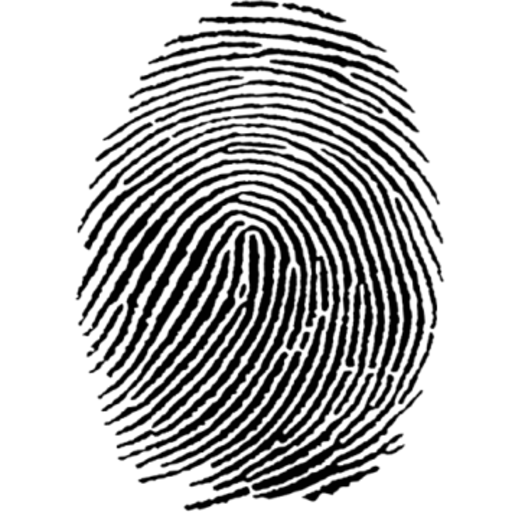
\includegraphics[width=\textwidth]{contenu/resources/images/fingerprint}
        \caption{Image originale}
    \end{subfigure}
    \hfill
    \begin{subfigure}[b]{.25\textwidth}
        \centering
        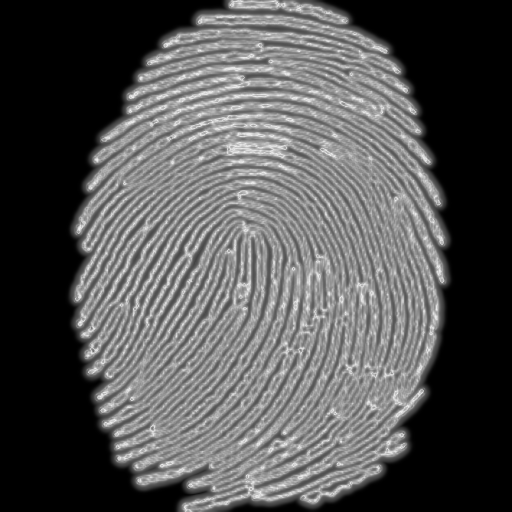
\includegraphics[width=\textwidth]{contenu/resources/images/pc_layer_0_1}
        \caption{Niveaux 0 et 1}
    \end{subfigure}
    \hfill
    \begin{subfigure}[b]{.25\textwidth}
        \centering
        
\includegraphics[width=\textwidth]{contenu/resources/images/pc_layer_2_depth-1}
        \caption{Niveaux 2 à $d-1$}
    \end{subfigure}

    \caption[Congruence de phases sur différents niveaux d'échelle]{Congruence de phases sur différents niveaux d'échelle. Conformément à notre intuition, on observe que sur les premiers niveaux (milieu), qui correspondent aux hautes fréquences, les détails fins ressortent, tandis que sur les derniers niveaux (droite), qui correspondent aux plus basses fréquences, c'est la structure globale, le contour de l'empreinte, qui apparait.}
    \label{fig:pc-selection-niveaux}
\end{figure}

Suite à cette observation, nous avons mis en place une méthode de sélection de niveaux de fréquences, pour pouvoir supprimer certains niveaux de la pyramide et observer l'effet sur la reconstruction. L'objectif était de pouvoir cibler les niveaux de structure qui nous intéressent et les extraire de l'image. Nous avons mis cela en application en faisant du filtrage de bandes de basses fréquences sur des textures de matériaux divers (voir figure~\ref{fig:filter-low-freq}), ce qui nous permet de \og gommer \fg{} les tâches présentes sur les images.

\begin{figure}
    \centering
    \begin{subfigure}[b]{.25\textwidth}
        \centering
        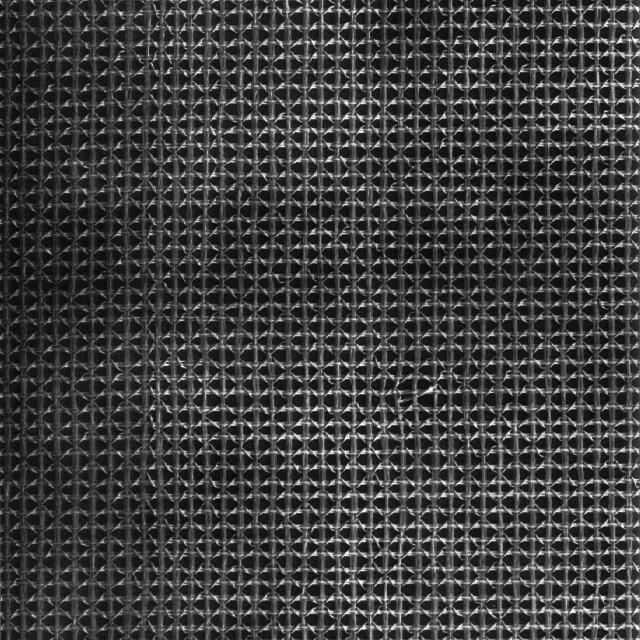
\includegraphics[width=\textwidth]{contenu/resources/images/lattice}
    \end{subfigure}
    \hspace{1em}
    \begin{subfigure}[b]{.25\textwidth}
        \centering
        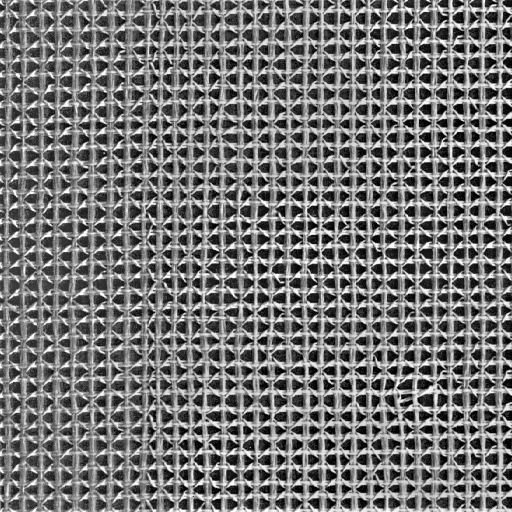
\includegraphics[width=\textwidth]{contenu/resources/images/lattice_filtered}
    \end{subfigure}
    \\
    \vspace{1em}
    \begin{subfigure}[b]{.25\textwidth}
        \centering
        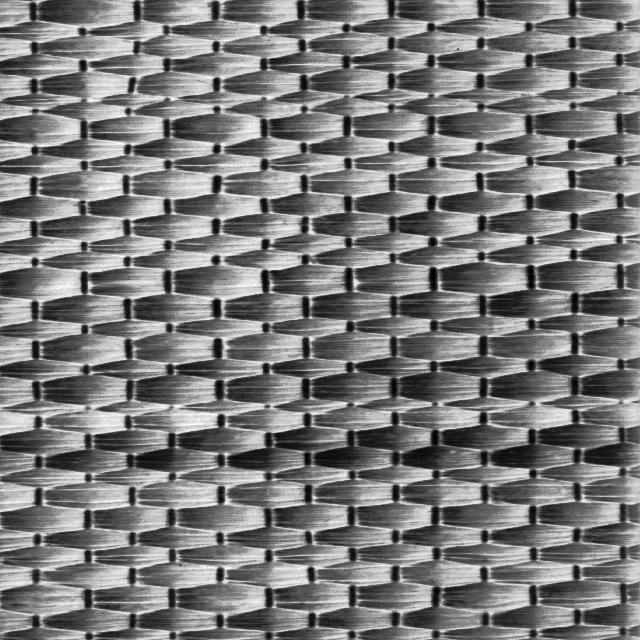
\includegraphics[width=\textwidth]{contenu/resources/images/lattice2}
    \end{subfigure}
    \hspace{1em}
    \begin{subfigure}[b]{.25\textwidth}
        \centering
        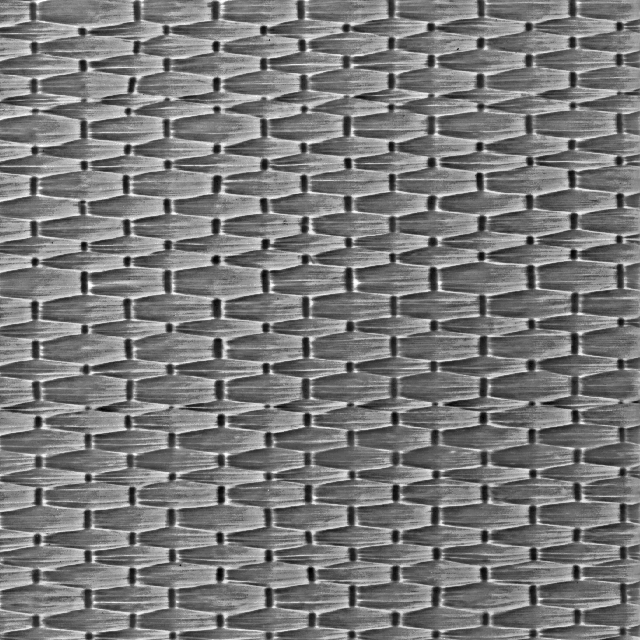
\includegraphics[width=\textwidth]{contenu/resources/images/lattice2_filtered}
    \end{subfigure}

    \caption[Filtrage de bandes de basses fréquences]{Filtrages de bandes de basses fréquences. Cette opération permet de supprimer les tâches présentes sur les textures, tout en conservant la structure globale et les détails. On voit les images originales (gauche) et les images reconstruites sans certains niveaux de la pyramide (droite). On garde typiquement les deux premiers niveaux, ainsi que le dernier, le résidu basse fréquence. Images tirées de la base de textures Brodatz~\cite{abdelmounaime_new_2013}.}
    \label{fig:filter-low-freq}
\end{figure}

\section{Synthèse de texture préservant la congruence de phase}

L'intérêt principal de notre cadre de travail est néanmoins l'utilisation de la congruence de phases, notamment en tant qu'indicatrice de la \textit{proximité} à un bord. La congruence de phases se comporte en effet comme un gradient dans la direction perpendiculaire au bord, et nous permet donc de savoir ponctuellement si un pixel se situe proche d'un bord.  Nous avons fait quelques expériences pour exploiter ce principe, puis nous avons mis au point une méthode de synthèse de textures pour traiter les textures à structure irrégulière.

Nous nous sommes inspirés de Lutz et al.~\cite{lutz_preserving_2023}, qui font le constat que les méthodes de synthèse par pavage apériodique, une sorte de synthèse par réorganisation reposant sur un échantillonnage uniforme de l'exemple d'entrée, échouent à préserver la fonction d'autocovariance de l'exemple. Des corrélations qui contribuent à préserver l'apparence de l'entrée sont ainsi mal reproduites, ce qui donne un air trop aléatoire au résultat. Pour remédier à cela, ils améliorent l'étape d'échantillonnage en utilisant le principe d' \og échantillonnage préférentiel \fg{}, qui consiste à influer l'échantillonnage en fonction d'une \og fonction de densité de probabilité \fg{}. En utilisant la fonction d'autocovariance comme densité de probabilité, ils montrent que l'on préserve mieux cette statistique et que l'on améliore la qualité de la synthèse.

Nous avons pensé appliquer cette idée à la congruence de phases. Le principe de la synthèse que nous proposons est d'adapter notre échantillonnage en fonction de l'endroit où l'on se situe dans la texture, afin de préserver la congruence de phase de l'exemple et ainsi conserver les contours et la structure de l'exemple. Pour créer du contenu inédit, nous remplaçons le contenu de la texture par du contenu qui possède propriétés similaires, notamment la congruence de phases, sous l'hypothèse que du contenu avec une congruence de phases similaire aura une apparence similaire. Pour notre application, nous avons choisi de travailler directement au niveau du pixel.

\subsection{Échantillonneur préservant la congruence de phase}

Pour mettre en place notre échantillonneur, on reprend la stratégie proposée par Pharr et al. dans leur livre~\cite{pharr_physically_2023}, qui utilise la méthode de la transformée inverse. Cette méthode d'échantillonnage repose sur le fait que pour échantillonner une variable aléatoire de loi donnée, il suffit d'échantillonner une variable aléatoire uniforme et d'appliquer la fonction de répartition inverse de la loi. Pour appliquer cette méthode, on commence par définir l'échantillonnage d'une fonction constante par morceaux 1D. Pour une fonction $f$ constante par morceaux :


\begin{equation}
    f(x) = \left\{
        \begin{array}{ll}
            v_0 & \mbox{si } x \in [x_0, x_1] \\
            v_1 & \mbox{si } x \in [x_1, x_2] \\
            \vdots & \vdots \\
            v_{N-1} & \mbox{si } x \in [x_{N-1}, x_N]
        \end{array}
    \right.
\end{equation}

d'intégrale $I$ :

\begin{equation}
    I = \int_{0}^{1} f(x) dx = \sum_{i=0}^{N-1} \frac{v_i}N,
\end{equation}

si on considère (sans perte de généralité) que $f$ est définie entre 0 et 1, et que les $x_i$ sont disposés de manière régulière $x_i = i / N$. La fonction de densité de probabilité associée à $f$ est alors simplement $p(x) = f(x) / I$. La fonction de répartition $F$ est alors linéaire par morceaux, définie aux $x_i$ :

\begin{equation}
    F(x_i) = \int_{0}^{x_i} p(t) dt = \sum_{j=0}^{x_i} \frac{v_j}{NI} = F(x_i-1) + \frac{v_i-1}{NI},
\end{equation}

et de coefficient directeur $v_i/I$ entre $x_i$ et $x_{i+1}$. On peut alors échantillonner $f$ en échantillonnant une variable aléatoire uniforme $u$ et en calculant $F^{-1}(u)$.

% TODO : figure pour la méthode d'inversion sur fonction constante par morceaux 1D

Il suffit ensuite de constater que nos textures sont des tableaux, donc des fonctions constantes par morceaux 2D, et que leur loi de probabilité conditionnelle et marginale sont des fonctions constantes par morceaux 1D. La stratégie est ainsi d'échantillonner la probabilité marginale pour avoir la première coordonnée, puis d'échantillonner la probabilité conditionnelle en utilisant la première valeur trouvée pour déterminer la deuxième coordonnée.

On va maintenant utiliser ce principe d'échantillonnage préférentiel pour préserver la fonction de congruence de phases. Pour cela, on veut pour chaque pixel tirer un nouveau pixel, avec une congruence de phases similaire. On voudrait avoir une fonction de densité de probabilité adaptée pour chaque valeur de congruence de phase, qui privilégie l'échantillonnage des valeurs autour de $x$ pour tout $x$ dans l'espace des valeurs de la PC, $[0, 1]$. Cependant la PC est à valeurs continues, il serait trop compliqué de stocker une fonction de densité pour chaque valeur. Pour résoudre ce problème, la PC est quantifiée en $N$ intervalles de taille constante $1/N$ de telle sorte que l'intervalle $i$ soit juste les valeurs de la PC entre $[i/N, (i+1)/N[$. Ce sont ces intervalles qui nous servent de densité de probabilité pour l'échantillonnage préférentiel. En pratique, on utilise $N=10$ et on partitionne en fait entre les valeurs minimum et maximum de la PC calculée, plutôt qu'entre 0 et 1, qui sont les extremums théoriques. Au moment de tirer du nouveau contenu, on regarde la valeur de PC du pixel que l'on cherche à remplacer, et on échantillonne avec la densité de probabilité correspondant à l'intervalle de PC dans lequel il se trouve.

% TODO : image des tranches de PC ?

- Les différentes classes, parler de nos textures typiques qui sont des tiles et un background

- le pré-calcul de la réalisation du sampler pour pouvoir faire l'échantillonnage depuis le shader. pose la question de quel offset utiliser.

- calcul de la spatially varying mean, utile plus tard pour le T\&B (besoin de parler de ça ??)

- résultats, montrer les réalisations du sampler (p-e ?)

% TODO mettre des subsubsection au dessus pour chaque partie du sampler ?

\subsection{Synthèse avec l'échantillonneur préférentiel}

Choix de la structure avec laquelle utiliser le sampler

- résultats (caca)

Pour ce faire, on procède en deux temps. Pour savoir quel contenu remplacer, et quelle est sa congruence de phase, pour aller chercher le nouveau contenu, il faut savoir où l'on se situe dans la texture, et quel est le contenu qui est attendu à cet endroit. On peut ici utiliser différentes techniques